\documentclass[12pt]{article}

\usepackage[utf8]{inputenc}
\usepackage{geometry}
\geometry{a4paper, margin=1in}
\usepackage{graphicx}
\usepackage{hyperref}
\usepackage{fancyhdr}

\setlength{\headheight}{15pt}
\pagestyle{fancy}
\fancyhf{}
\rhead{Computer Workshop Course}
\rfoot{Page \thepage}
\title{
	\vspace{2in}
	\textbf{Final Project}\\
	\vspace{.2 in}
	\large Iran University of Science and Technology\\
	\large Department of Computer Engineering\\
	\vspace{2in}
}
\author{
	\vspace{0.2in}
	Nazanin Sharifi\\
	Computer Workshop 
	\vspace{0.2in}
}
\date{ Bahman 1402}

\begin{document}
	\begin{titlepage}
	\maketitle
	\thispagestyle{empty}
\end{titlepage}
\newpage
\tableofcontents
\newpage
\section{Git and GitHub}
\subsection{Repository Initialization and Commits}
1.Create a new GitHub repository:

- Go to the GitHub website (https://github.com) and log in to your account.

- Click on the "+" button in the top right corner and select "New repository" from the dropdown menu.

- Give your repository a name and an optional description.

- Choose  the repository to be public and add a README file.\\
2. Clone the repository to your local machine:

- Open a terminal or command prompt on your local machine.

- Navigate to the directory where you want to clone the repository.

- Run the following command, replacing "repository-url" with the URL of your GitHub repository:

git clone repository-url\\
3. Write your assignment document in LaTeX:\\
4. Commit and push your changes:

- Open a terminal or command prompt in the cloned repository directory.

- Run the following commands to stage and commit your changes:

git add .

git commit -m "Initial commit"



- Run the following command to push your changes to the remote repository on GitHub:

git push origin master

\subsection{GitHub Actions for LaTeX Compilation}
Set up GitHub Actions for automatic PDF compilation:

- In GitHub repository, click on the "Actions" tab.

- Click on the "Set up a workflow yourself" link.

- Replace the default YAML code with the main.yml.

- Click on the "Start commit" button, provide a commit message, and click on the "Commit new file" button.\\
Now, whenever push a tag to  GitHub repository, GitHub Actions will automatically compile  LaTeX document to a PDF and can download the compiled PDF from the "Actions" tab.

\section{Exploration Tasks}
\subsection{Vim Advanced Features}
1. Macros:

Vim macros allow you to record a series of keystrokes and replay them later. This can be very useful for automating repetitive tasks. To start recording a macro, press q followed by a key of your choice (e.g., q1). Then perform the desired actions or commands. To stop recording, press q again. To replay the macro, use @ followed by the key you used to start recording (e.g., @1).\\
2. Registers:

Vim registers are like storage spaces where you can copy and paste text or yank and put text. Vim provides multiple registers, each identified by a letter. The default register is ", but you can also use other letters like a, b, etc. To copy text to a register, visually select the text and use "ay where a is the register letter. To paste from a register, use "ap where a is the register letter.\\
3. Persistent Undo:

Vim's persistent undo feature allows you to undo changes even after closing and reopening a file. By default, Vim doesn't enable this feature, but you can set it up by adding the following lines to your vimrc file:

set undofile

set undodir=~/.vim/undo\\
With this configuration, Vim will store undo history in the specified undodir (change it to a directory of your choice) and you can use the :undo command to navigate and undo changes made in previous sessions.
\subsection{Memory profiling}

Dynamic memory allocation in C allows us to allocate memory at runtime, which means that memory can be allocated and deallocated as needed during the execution of a program. This is in contrast to static memory allocation, where memory is allocated at compile-time and remains fixed throughout the program's execution.\\
The C programming language provides several functions for dynamic memory allocation, including malloc(), calloc(), realloc(), and free(). These functions are included in the stdlib.h header file.\\
Here is a brief explanation of each function:



1. malloc(): This function is used to dynamically allocate memory in C. It takes the number of bytes to be allocated as its argument and returns a pointer to the allocated memory. If the memory allocation is successful, the pointer points to the beginning of the allocated memory block. If the allocation fails, NULL is returned.



2. calloc(): This function is similar to malloc(), but it additionally initializes the allocated memory to zero. It takes two arguments - the number of elements to allocate and the size of each element. The total memory allocated is equal to the product of these two arguments. Like malloc(), calloc() returns a pointer to the allocated memory or NULL on failure.



3. realloc(): This function is used to change the size of the previously allocated memory block. It takes two arguments - a pointer to the previously allocated memory block and the new size in bytes. If the reallocation is successful, the pointer to the newly allocated memory block is returned. If the reallocation fails, NULL is returned. If the new size is smaller than the original size, the excess memory is freed.



4. free(): This function is used to deallocate the dynamically allocated memory. It takes a pointer to the memory block as its argument and frees the memory for reuse.\vspace{.1 in}
Dynamic memory allocation is useful when we don't know the exact amount of memory needed at compile-time or when memory requirements may change during program execution. It allows for efficient memory utilization and flexibility in managing memory resources. However, it is important to properly deallocate the allocated memory to avoid memory leaks and optimize memory usage.
\subsubsection{Memory Leak}
Memory leaks occur when a program fails to release memory that is no longer needed, resulting in wasted memory resources. When a program creates objects or allocates memory dynamically, it should release them when they are no longer required. If this release doesn't happen, a memory leak occurs.\\
Memory leaks can happen in a program due to various reasons, including:

1. Forgetting to deallocate memory: When dynamically allocated memory is not freed with the appropriate deallocation function (e.g., delete in C++ or free in C), a memory leak can occur.

2. Incorrect logic: If the program flow or logic doesn't properly handle all scenarios where memory should be deallocated, memory leaks can happen.

3. Unreachable objects: If objects are created but become unreachable or lose their references without being deallocated, memory leaks can occur.

4. Circular references: In languages with garbage collection, if two or more objects reference each other, but no other parts of the program reference them, the garbage collector may fail to recognize them as unused, causing a leak.\\
Overall, memory leaks occur when memory is allocated but not properly released, leading to a gradual loss of available memory and potential performance issues in the program.
\subsubsection{Memory profilers}
Valgrind is an open-source programming tool suite that assists in debugging, profiling, and optimizing software, primarily focused on memory management. It is widely used by developers to detect memory leaks, memory errors, and other memory-related issues in C, C++, and other languages.



The main purpose of Valgrind is to provide a framework for executing programs in a controlled environment, where it can monitor and track memory usage, identify potential memory leaks, and report errors. Valgrind achieves this by dynamically instrumenting the program's binary code, allowing it to intercept memory allocations, deallocations, and accesses during runtime.



When memory leaks occur, Valgrind acts as a powerful aid in identifying and fixing those issues. Memory leaks happen when dynamically allocated memory is not properly deallocated, leading to a gradual consumption of system resources. These leaks can cause significant problems, such as increased memory usage, reduced performance, and even program crashes.



Valgrind's core tool, called Memcheck, is particularly useful for detecting and diagnosing memory leaks. Memcheck performs thorough analysis of memory usage and tracks every allocation and deallocation in the program, ensuring that all allocated memory is correctly released. It identifies memory leaks by monitoring which memory blocks were not freed before the program's termination.



When Valgrind detects a memory leak, it provides detailed reports indicating the exact location in the code where the memory was allocated but not freed. It highlights the call stack, pointing to the source code line responsible for the allocation, making it easier for developers to identify and fix the issue.



Furthermore, Valgrind offers additional tools like Helgrind (for detecting thread synchronization issues), Cachegrind (for cache profiling), and Callgrind (for call-graph profiling). These tools provide further insights into program behavior and performance, helping developers optimize their code and identify potential bottlenecks.



Overall, Valgrind is a valuable tool for programmers as it helps prevent memory leaks and memory errors, improving the stability and performance of software. Its comprehensive analysis capabilities, combined with easy-to-understand reports, make it an essential tool in the debugging and optimization process, ultimately leading to more reliable and efficient code.

\subsection{GNU/Linux Bash Scripting}
\subsubsection{fzf}
\begin{itemize}
	\item Fuzzy searching is a technique used in information retrieval to find items that may not exactly match the search query but are similar in some way. It involves searching for approximate matches based on patterns, similarities, or partial matches rather than exact matches.
	\item The command "\texttt{ls | fzf}" is used to enhance the functionality of the "ls" command. It pipes the output of the "ls" command (which lists files and directories in the current directory) into fzf. Fzf then provides an interactive fuzzy search interface where you can search for files or directories by typing a query. The search results are displayed in real-time, allowing you to select and navigate through the results efficiently.
	
\end{itemize}

\subsubsection{Using fzf to find your favorite PDF}
1. To list the directory of all the files with the extension .PDF, you can use the following command:\\

\textbf{fd -e pdf}\\
\\This command uses the fd command, which is a faster and more user-friendly alternative to the traditional find command. The -e flag is used to specify the file extension, in this case, "pdf".\\
2. To use fzf to select a PDF from the data gathered above, you can pipe the output of the previous command into fzf. Here's an example command:\\


\textbf{fd -e pdf | fzf}\\
\\This command will display a fuzzy search interface using fzf, allowing you to search and select a PDF file from the list generated by the fd command. Once you select a file, it will be printed to the console.

\subsubsection{Opening the file using Zathura}
To open the selected PDF file using Zathura, you can use the following command:\\

\texttt{zathura "\$(\textit{fd -e pdf | fz})"}\\
\\This command uses the \$(command) syntax to execute the command inside the parentheses and pass its output as an argument to the zathura command. The fd -e pdf | fzf command generates a list of PDF files using fd and filters it through fzf, allowing you to select a file. The selected file is then passed as an argument to the zathura command, which opens it in Zathura.

\section{Git and FOSS}
\subsection{Issues}

\begin{figure}[h]
    \centering
    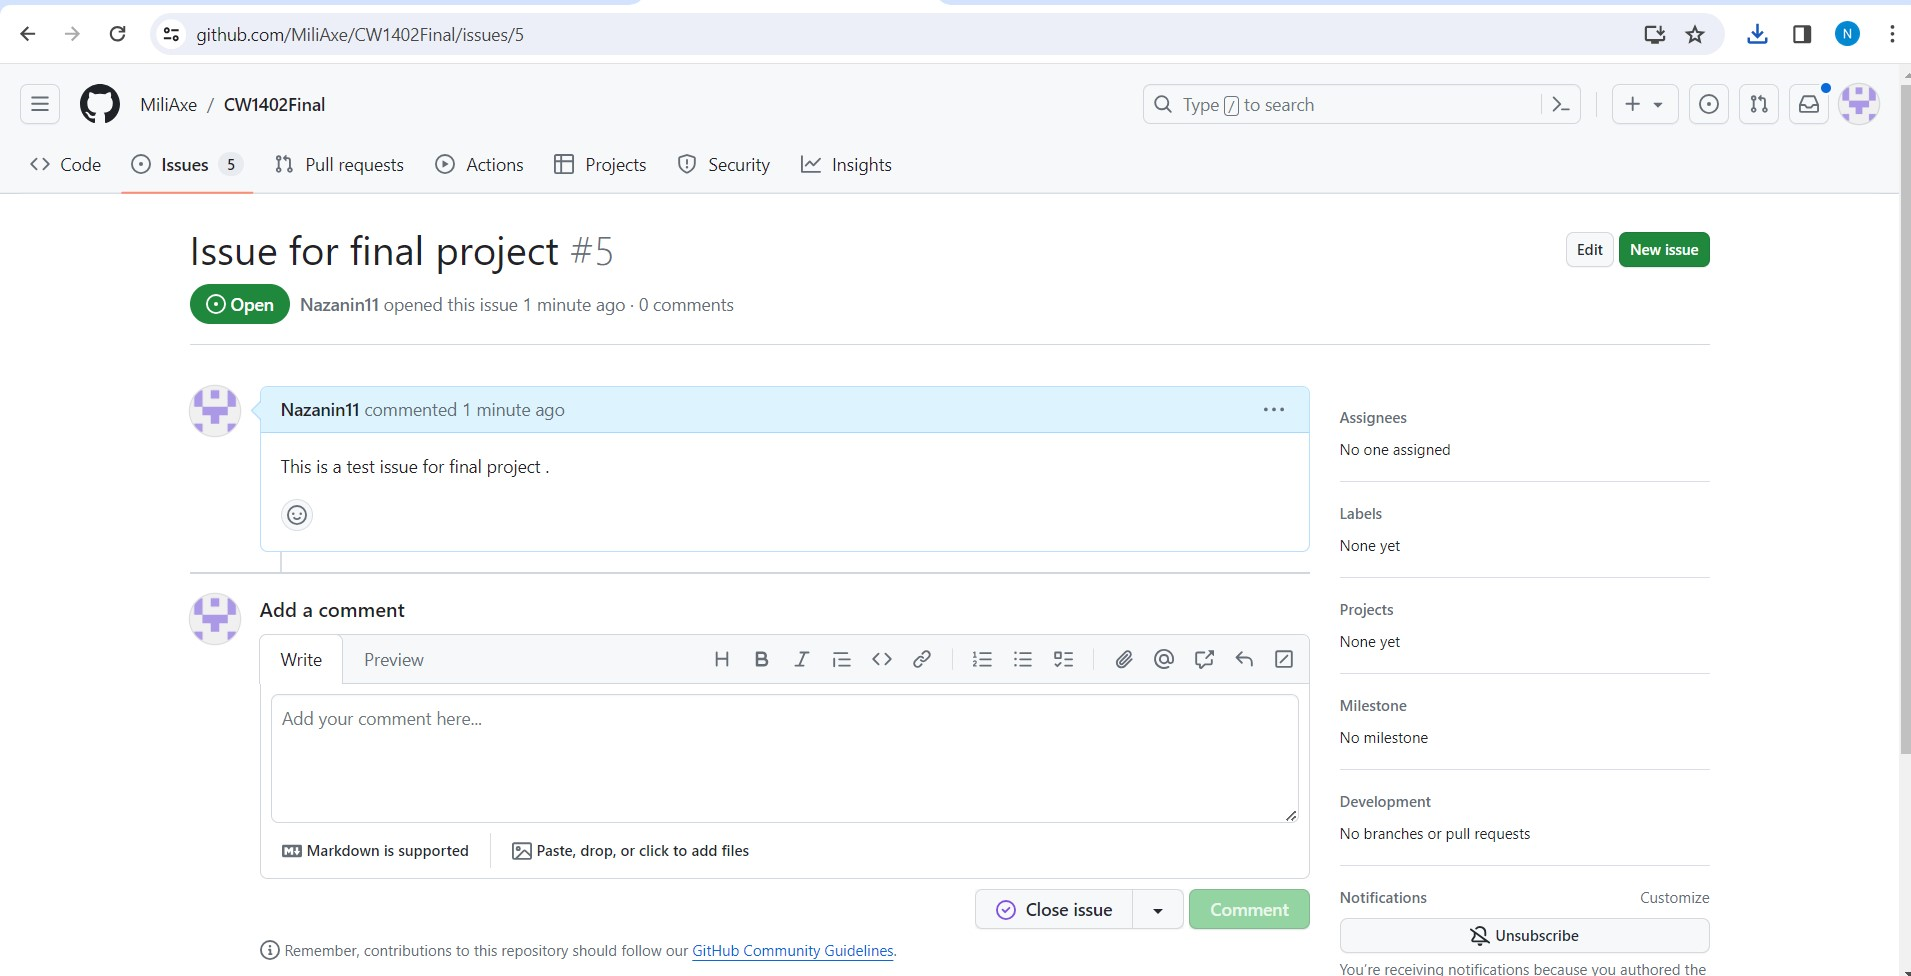
\includegraphics[width=0.6\linewidth]{Screenshot}
	\caption{This is just a test}
	
\end{figure}



\end{document}	
	
	
